% layout for presentations with table of contents
\documentclass{beamer}
\usepackage{graphicx,color,fancybox,pifont}
\usepackage{hyperref}
\hypersetup{colorlinks=true}%, urlcolor=blue}
% basic theme
\usetheme{Madrid}

% define DESY specific colours
\definecolor{desycyan}{rgb}{0.000,0.651,0.922}
\definecolor{desyorange}{rgb}{0.949,0.557,0.00}
\definecolor{desygray}{rgb}{0.467,0.467,0.467}

% change colours to desy style
\setbeamercolor{title}{fg=white,bg=desycyan}
\setbeamercolor{title bar}{fg=white,bg=desycyan}
\setbeamercolor{frametitle}{fg=white,bg=desycyan}
\setbeamercolor{section in head/foot}{fg=white,bg=desycyan}
\setbeamercolor{subsection in head/foot}{fg=desycyan,bg=white}
\setbeamercolor{normal text}{fg=black,bg=white}

% set toc
\setbeamercolor{section in toc}{fg=black}
\setbeamercolor{subsection in toc}{fg=black}
\setbeamercolor{section number projected}{fg=white,bg=desyorange}
\setbeamercolor{subsection number projected}{fg=white,bg=desyorange}
\setbeamertemplate{sections/subsections in toc}[square]

% set itemize environments
\setbeamercolor{description item}{fg=desyorange}
\setbeamercolor{enumerate item}{fg=desyorange}
\setbeamercolor{itemize item}{fg=desyorange}
\setbeamertemplate{itemize item}{\color{desyorange}{\ding{228}}}
\setbeamertemplate{itemize subitem}{\color{desygray}{\tiny{\ding{110}}}}

% set block environments
\setbeamercolor{block title}{fg=white,bg=desycyan}

% add page numbers
\setbeamertemplate{footline}[frame number]

% settings for boxes
\cornersize*{4mm}

% remove navigation symbols on all slides
\beamertemplatenavigationsymbolsempty


%Relative path for images
\graphicspath{{../Images/}{./week16/}}


% data for titlepage
\title[Data Monitoring]{2012 Data Monitoring for Top Group}
\author[Ivan Asin\inst{1}]{\underline{Ivan Asin}\inst{1}, Abideh Jafari\inst{2} and Enrique Palencia\inst{3}}
\date{2012-04-26}
\institute[DESY]{
	\inst{1} DESY\\
	\inst{2} School of Particles and Accelerator Inst. for Res. in Fundam. S.\\
	\inst{3} CERN
}

\titlegraphic{
\hspace{1cm}\includegraphics[width=1.5cm, height=1.5cm]{desyLogo.pdf}
\hspace{6cm}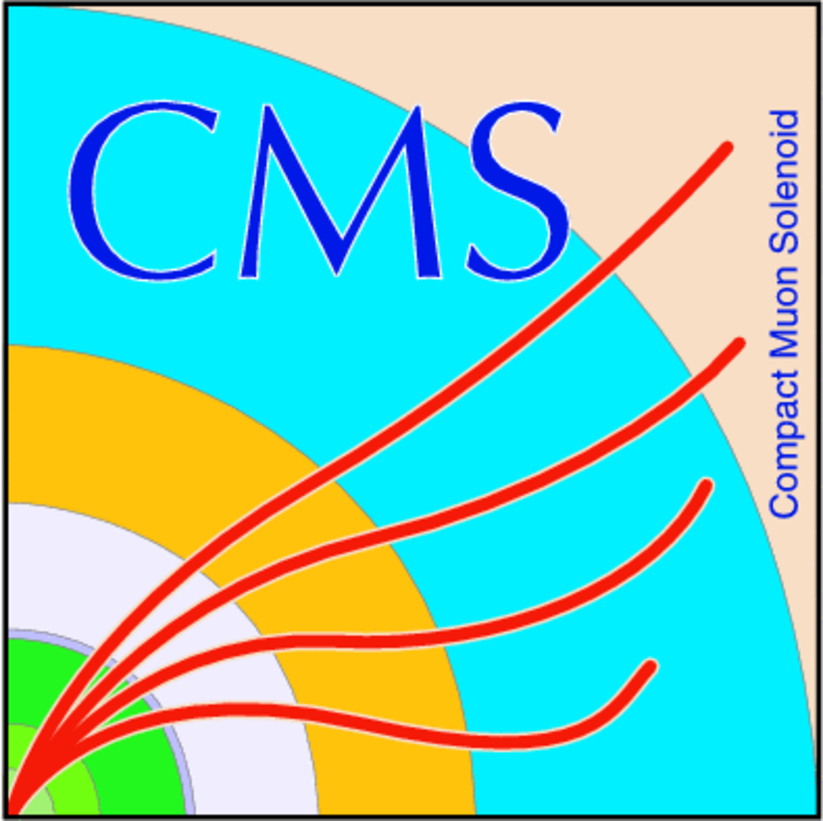
\includegraphics[width=1.5cm, height=1.5cm]{CMSlogo.pdf}
}

\begin{document}

\begin{frame}
 \titlepage
\end{frame}


%\begin{frame}
%\frametitle{Introduction}
%\begin{itemize}
%\item Selection criteria interesting for the Top Group (feedback always welcome)
% \item What will be presented later:
% \begin{itemize}
% \item Certified data comparison of consecutive weeks
% \item Certified VS Non Certified data of the same week
% \end{itemize}
% \item Common features
% \begin{itemize}
% \item CMSSW\_5\_2\_3\_patch4
% \item DQM/Physics  (V00-03-15)
% \item Dataset: $l+jets$
% \begin{itemize}
% \item /SingleMu/Run2012A-PromptReco-v1/AOD
% \item /SingleElectron/Run2012A-PromptReco-v1/AOD\\
% \end{itemize}
%\item Golden JSON\footnote{\href{https://cms-service-dqm.web.cern.ch/cms-service-dqm/CAF/certification/Collisions12/8TeV/Prompt/Cert_190456-191276\_8TeV\_PromptReco\_Collisions12\_JSON.txt}{$Cert\_190456-191276\_8TeV\_PromptReco\_Collisions12\_JSON.txt$}}
%\begin{itemize}
%\item Week 2012/Apr/7-13: 190456-190688 (week 15)
%\item Week 2012/Apr/14-20: 190689-191276 (week 16)
%\end{itemize}
%\item Non Certified\footnote{\url{https://cms-service-dqm.web.cern.ch/cms-service-dqm/CAF/certification/Collisions12/8TeV/DCSOnly/json_DCSONLY.txt}}
%\begin{itemize}
%\item Runs: 191277-191939
%\end{itemize}
% \end{itemize}
% \end{itemize}
% \end{frame}


\begin{frame}
\frametitle{Introduction}
Common features
\begin{itemize}
\item CMSSW\_5\_2\_3\_patch4
\item DQM/Physics  (V00-03-15)
\item Dataset: $l+jets$
\begin{itemize}
\item /SingleMu/Run2012A-PromptReco-v1/AOD
\item /SingleElectron/Run2012A-PromptReco-v1/AOD\\
\end{itemize}
\end{itemize}
\end{frame}





% \begin{frame}
% \frametitle{Loose Working Point}
% Primary Vertex: $|d_X|<1.0$ cm, $|d_Y|<1.0$ cm, $|d_Z|<20.0$ cm, $>$3 hits
% \begin{columns}[c]
% \column{5cm}
% \center{Muons}
% \begin{itemize}
% \item Global Muon
% \item $>10$ tracker hits
% \item $\chi^2/{ndf}<10$
% %\item $I=\frac{p_T^{0.3}+E^{0.3}+H^{0.3}}{p_T}<0.1$
% \item $p_T>10GeV$
% \item $|\eta|<2.1$
% \item $>1$ muon
% \end{itemize}
% \column{5cm}
% \center{Jets}
% \begin{itemize}
% \item ak5Calo Jets
% \item$p_T>15 GeV$
% \item $|\eta|<2.5$
% \item $E/H>0.1$
% \end{itemize}
% \begin{itemize}
% \item $TCHE>1.25$
% \item $TCHP>3.00$
% \item $SSVHE>2.05$
% \item $>1$, $>2$, $>3$, $>4$ jets
% \end{itemize}
% \end{columns}
% \end{frame}


\begin{frame}
\frametitle{Medium Working Point}
Primary Vertex: $|d_X|<1.0$ cm, $|d_Y|<1.0$ cm, $|d_Z|<20.0$ cm, $>$3 hits
\begin{columns}[c]
\column{4cm}
\center{Muons}
\begin{itemize}
\item Global Muon
\item $>10$ tracker hits
\item $\chi^2/{ndf}<10$
\item $\frac{p_T^{0.3}+E^{0.3}+H^{0.3}}{p_T}<0.1$
\item $p_T>20GeV$
\item $|\eta|<2.1$
%\item $>1$ muon
\end{itemize}
\column{4.5cm}
\center{Electrons}
\begin{itemize}
%\item gsfElectrons
\item simpleEleId70cIso
\item $\frac{p_{T\, Trk.}^{0.3}+E^{0.3}+H^{0.3}}{p_T}<0.1$
\item $p_T>25GeV$
\item $|\eta|<2.5$
\end{itemize}
\column{4cm}
\center{Jets}
\begin{itemize}
\item ak5Calo
\item$p_T>15 GeV$
\item $|\eta|<2.5$
\item $E/H>0.1$
\end{itemize}
\begin{itemize}
\item $TCHE>1.25$
\item $TCHP>3.00$
\item $SSVHE>2.05$
%\item $>1$, $>2$, $>3$, $>4$ jets
\end{itemize}
\end{columns}
\end{frame}

\begin{frame}
\frametitle{Plots}
Next plots are the comparison of the Certified\footnote{Golden JSON: \href{https://cms-service-dqm.web.cern.ch/cms-service-dqm/CAF/certification/Collisions12/8TeV/Prompt/Cert_190456-191276\_8TeV\_PromptReco\_Collisions12\_JSON.txt}{$Cert\_190456-191276\_8TeV\_PromptReco\_Collisions12\_JSON.txt$}} runs:
\begin{itemize}
\item Runs 190456-190688: $L\simeq 609/nb$ ($\mu+jet$) taken between Apr/5-8
\item Runs 190689-191276: $L\simeq 283/pb$ ($\mu+jet$) taken between Apr/8-15
\end{itemize}
Selection
\begin{itemize}
\item 1 muon
\item 1 muon + 4 jets
\end{itemize}
\begin{itemize}
\item To note: \textbf{ALL} plots are normalized to unit area
\end{itemize}
\end{frame}



%---------------------------------------------------------------------------------------------------
%********* CertVSCert SingleMuon Medium step0 ***********

\begin{frame}
\frametitle{Certified VS Certified: 1 Muon Requested}
\hspace{-0.7cm}
\includegraphics[scale=0.21]{week16/CertVSCert/TopSingleMuonMediumDQM_step0PvMult.pdf}
\includegraphics[scale=0.21]{week16/CertVSCert/TopSingleMuonMediumDQM_step0MuonEta.pdf}
\includegraphics[scale=0.21]{week16/CertVSCert/TopSingleMuonMediumDQM_step0MuonPt.pdf}\\
\hspace{-0.7cm}
\includegraphics[scale=0.21]{week16/CertVSCert/TopSingleMuonMediumDQM_step0MuonRelIso.pdf}
\includegraphics[scale=0.21]{week16/CertVSCert/TopSingleMuonMediumDQM_step0Jet1Pt.pdf}
\includegraphics[scale=0.21]{week16/CertVSCert/TopSingleMuonMediumDQM_step0JetMult.pdf}
\end{frame}


\begin{frame}
\frametitle{Certified VS Certified: 1 Muon + 4 Jets Requested}
\hspace{-0.7cm}
\includegraphics[scale=0.21]{week16/CertVSCert/TopSingleMuonMediumDQM_step4PvMult.pdf}
\includegraphics[scale=0.21]{week16/CertVSCert/TopSingleMuonMediumDQM_step4MuonEta.pdf}
\includegraphics[scale=0.21]{week16/CertVSCert/TopSingleMuonMediumDQM_step4MuonPt.pdf}\\
\hspace{-0.7cm}
\includegraphics[scale=0.21]{week16/CertVSCert/TopSingleMuonMediumDQM_step4JetBDiscVtx.pdf}
\includegraphics[scale=0.21]{week16/CertVSCert/TopSingleMuonMediumDQM_step4MassTop.pdf}
\includegraphics[scale=0.21]{week16/CertVSCert/TopSingleMuonMediumDQM_step4MassW.pdf}
\end{frame}

% \begin{frame}
% \frametitle{Certified VS Certified: 1 Electron Requested}
% \hspace{-0.7cm}
%\includegraphics[scale=0.21]{week16/CertVSCert/TopSingleElectronMediumDQM_step0PvMult.pdf}
% \includegraphics[scale=0.21]{week16/CertVSCert/TopSingleElectronMediumDQM_step0ElecEta.pdf}
% \includegraphics[scale=0.21]{week16/CertVSCert/TopSingleElectronMediumDQM_step0ElecPt.pdf}\\
% \hspace{-0.7cm}
%\includegraphics[scale=0.21]{week16/CertVSCert/TopSingleElectronMediumDQM_step0ElecRelIso.pdf}
% \includegraphics[scale=0.21]{week16/CertVSCert/TopSingleElectronMediumDQM_step0Jet1Pt.pdf}
% \includegraphics[scale=0.21]{week16/CertVSCert/TopSingleElectronMediumDQM_step0JetMult.pdf}
% \end{frame}
% 
% 
% \begin{frame}
% \frametitle{Certified VS Certified: 1 Electron + 4 Jets Requested}
% \hspace{-0.7cm}
% \includegraphics[scale=0.21]{week16/CertVSCert/TopSingleElectronMediumDQM_step4PvMult.pdf}
% \includegraphics[scale=0.21]{week16/CertVSCert/TopSingleElectronMediumDQM_step4ElecEta.pdf}
% \includegraphics[scale=0.21]{week16/CertVSCert/TopSingleElectronMediumDQM_step4ElecPt.pdf}\\
% \hspace{-0.7cm}
% \includegraphics[scale=0.21]{week16/CertVSCert/TopSingleElectronMediumDQM_step4JetBDiscVtx.pdf}
% \includegraphics[scale=0.21]{week16/CertVSCert/TopSingleElectronMediumDQM_step4MassTop.pdf}
% \includegraphics[scale=0.21]{week16/CertVSCert/TopSingleElectronMediumDQM_step4MassW.pdf}
% \end{frame}
% 
% 

%---------------------------------------------------------------------------------------------------
\begin{frame}
\frametitle{Certified VS Non-Certified}
Certified\footnote{Golden JSON: \href{https://cms-service-dqm.web.cern.ch/cms-service-dqm/CAF/certification/Collisions12/8TeV/Prompt/Cert_190456-191276\_8TeV\_PromptReco\_Collisions12\_JSON.txt}{$Cert\_190456-191276\_8TeV\_PromptReco\_Collisions12\_JSON.txt$}} runs:
\begin{itemize}
\item Runs 190689-191276: taken between 2012/Apr/8-15
\begin{itemize}
\item $L\simeq 283/pb$ ($\mu+jet$)
\item $L\simeq 276/pb$ ($e+jet$)
\end{itemize}
\end{itemize}
Non Certified\footnote{\url{https://cms-service-dqm.web.cern.ch/cms-service-dqm/CAF/certification/Collisions12/8TeV/DCSOnly/json_DCSONLY.txt}} runs:
\begin{itemize}
\item Runs 191277-191939: taken between 2012/Apr/15-21
\begin{itemize}
\item $L\simeq 293/pb$ ($\mu+jet$)
\item $L\simeq 254/pb$ ($e+jet$)
\end{itemize}
\end{itemize}
Selection
\begin{itemize}
\item 1 lepton
\item 1 lepton + 4 jets
\end{itemize}
\begin{itemize}
\item To note: \textbf{ALL} plots are normalized to unit area
\end{itemize}
\end{frame}


%********* CertVSNCert SingleMuon Medium step0 ***********

\begin{frame}
\frametitle{Certified VS Not-Certified: 1 Muon Requested}
\hspace{-0.7cm}
\includegraphics[scale=0.21]{week16/CertVSNCert/TopSingleMuonMediumDQM_step0PvMult.pdf}
\includegraphics[scale=0.21]{week16/CertVSNCert/TopSingleMuonMediumDQM_step0MuonEta.pdf}
\includegraphics[scale=0.21]{week16/CertVSNCert/TopSingleMuonMediumDQM_step0MuonPt.pdf}\\
\hspace{-0.7cm}
\includegraphics[scale=0.21]{week16/CertVSNCert/TopSingleMuonMediumDQM_step0MuonRelIso.pdf}
\includegraphics[scale=0.21]{week16/CertVSNCert/TopSingleMuonMediumDQM_step0Jet1Pt.pdf}
\includegraphics[scale=0.21]{week16/CertVSNCert/TopSingleMuonMediumDQM_step0JetMult.pdf}
\end{frame}


\begin{frame}
\frametitle{Certified VS Not-Certified: 1 Muon + 4 Jets Requested}
\hspace{-0.7cm}
\includegraphics[scale=0.21]{week16/CertVSNCert/TopSingleMuonMediumDQM_step4PvMult.pdf}
\includegraphics[scale=0.21]{week16/CertVSNCert/TopSingleMuonMediumDQM_step4MuonEta.pdf}
\includegraphics[scale=0.21]{week16/CertVSNCert/TopSingleMuonMediumDQM_step4MuonPt.pdf}\\
\hspace{-0.7cm}
\includegraphics[scale=0.21]{week16/CertVSNCert/TopSingleMuonMediumDQM_step4JetBDiscVtx.pdf}
\includegraphics[scale=0.21]{week16/CertVSNCert/TopSingleMuonMediumDQM_step4MassTop.pdf}
\includegraphics[scale=0.21]{week16/CertVSNCert/TopSingleMuonMediumDQM_step4MassW.pdf}
\end{frame}

\begin{frame}
\frametitle{Certified VS Not-Certified: 1 Electron Requested}
\hspace{-0.7cm}
\includegraphics[scale=0.21]{week16/CertVSNCert/TopSingleElectronMediumDQM_step0PvMult.pdf}
\includegraphics[scale=0.21]{week16/CertVSNCert/TopSingleElectronMediumDQM_step0ElecEta.pdf}
\includegraphics[scale=0.21]{week16/CertVSNCert/TopSingleElectronMediumDQM_step0ElecPt.pdf}\\
\hspace{-0.7cm}
\includegraphics[scale=0.21]{week16/CertVSNCert/TopSingleElectronMediumDQM_step0ElecRelIso.pdf}
\includegraphics[scale=0.21]{week16/CertVSNCert/TopSingleElectronMediumDQM_step0Jet1Pt.pdf}
\includegraphics[scale=0.21]{week16/CertVSNCert/TopSingleElectronMediumDQM_step0JetMult.pdf}
\end{frame}


\begin{frame}
\frametitle{Certified VS Not-Certified: 1 Electron + 4 Jets Requested}
\hspace{-0.7cm}
\includegraphics[scale=0.21]{week16/CertVSNCert/TopSingleElectronMediumDQM_step4PvMult.pdf}
\includegraphics[scale=0.21]{week16/CertVSNCert/TopSingleElectronMediumDQM_step4ElecEta.pdf}
\includegraphics[scale=0.21]{week16/CertVSNCert/TopSingleElectronMediumDQM_step4ElecPt.pdf}\\
\hspace{-0.7cm}
\includegraphics[scale=0.21]{week16/CertVSNCert/TopSingleElectronMediumDQM_step4JetBDiscVtx.pdf}
\includegraphics[scale=0.21]{week16/CertVSNCert/TopSingleElectronMediumDQM_step4MassTop.pdf}
\includegraphics[scale=0.21]{week16/CertVSNCert/TopSingleElectronMediumDQM_step4MassW.pdf}
\end{frame}




\begin{frame}
\frametitle{Conclusions}
\begin{itemize}
\item More plots available in the GUI\footnote{\url{http://pccms94.cern.ch:8888/dqm/devtest/}}
\item Lepton+jets monitoring tools set up and working%: Loose and Medium working points.
\begin{itemize}
 \item Dilepton samples and plots are a ``work in progress''
\end{itemize}
\item Nothing worrying seen in data
\item Weekly data monitoring but bi-weekly report in this meeting.
\begin{itemize}
\item If you are interested in the weekly ``evolution'' check to the TWiki\footnote{\url{https://twiki.cern.ch/twiki/bin/view/CMS/TWikiTopQuarkComWG4Operations}}
\end{itemize}
\item If you are interested in monitoring some particular variable, certain cuts,\ldots please contact Abideh, Enrique or Ivan
\end{itemize}

\end{frame}



\end{document}
